

\tikzset{every picture/.style={line width=0.75pt}} %set default line width to 0.75pt

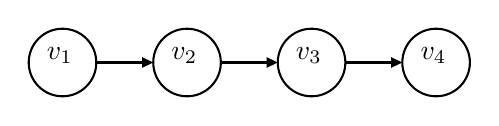
\begin{tikzpicture}[x=0.75pt,y=0.75pt,yscale=-1,xscale=1]
%uncomment if require: \path (0,66); %set diagram left start at 0, and has height of 66


% Text Node
\draw    (30, 31) circle [x radius= 16.28, y radius= 16.28]   ;
\draw (21,22.4) node [anchor=north west][inner sep=0.75pt]    {$v_{1}$};
% Text Node
\draw    (90, 31) circle [x radius= 16.28, y radius= 16.28]   ;
\draw (81,22.4) node [anchor=north west][inner sep=0.75pt]    {$v_{2}$};
% Text Node
\draw    (150, 31) circle [x radius= 16.28, y radius= 16.28]   ;
\draw (141,22.4) node [anchor=north west][inner sep=0.75pt]    {$v_{3}$};
% Text Node
\draw    (210, 31) circle [x radius= 16.28, y radius= 16.28]   ;
\draw (201,22.4) node [anchor=north west][inner sep=0.75pt]    {$v_{4}$};
% Connection
\draw    (46.28,31) -- (70.72,31) ;
\draw [shift={(73.72,31)}, rotate = 180] [fill={rgb, 255:red, 0; green, 0; blue, 0 }  ][line width=0.08]  [draw opacity=0] (5.36,-2.57) -- (0,0) -- (5.36,2.57) -- cycle    ;
% Connection
\draw    (106.28,31) -- (130.72,31) ;
\draw [shift={(133.72,31)}, rotate = 180] [fill={rgb, 255:red, 0; green, 0; blue, 0 }  ][line width=0.08]  [draw opacity=0] (5.36,-2.57) -- (0,0) -- (5.36,2.57) -- cycle    ;
% Connection
\draw    (166.28,31) -- (190.72,31) ;
\draw [shift={(193.72,31)}, rotate = 180] [fill={rgb, 255:red, 0; green, 0; blue, 0 }  ][line width=0.08]  [draw opacity=0] (5.36,-2.57) -- (0,0) -- (5.36,2.57) -- cycle    ;

\end{tikzpicture}